\chapter{Exercise 9}
\label{cha:ugeopgave-9}

The purpose of this exercise is to understand and implement planar reflections using OpenGL.


\section{Part 1}

Completion of this part is considered as a future work.

\section{Part 2}

When I comment out the line that renders the plane in the \emph{drawPlane()} function, the resulting scene is Figure \ref{fig:9-2}.

\begin{figure}[hp]
\centering
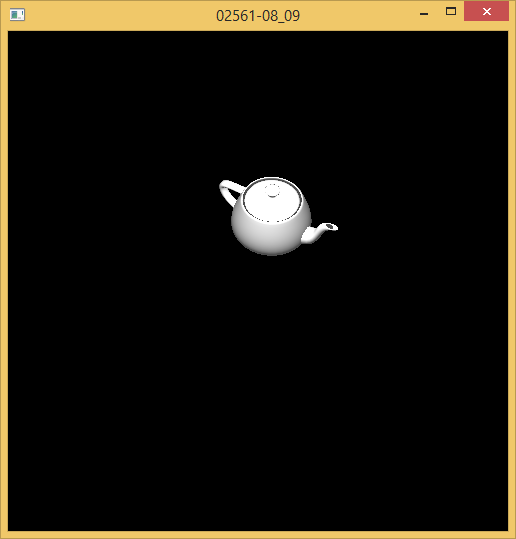
\includegraphics[width=8cm]{../Screenshots/ex-9b/2.png}
\caption{The scene without the plane being rendered}
\label{fig:9-2}
\end{figure}

\section{Part 3}

By following the steps described in exercise text document, I manage to display a reflected teapot in the scene (see Figure \ref{fig:9-3}).

\begin{figure}[hp]
\centering
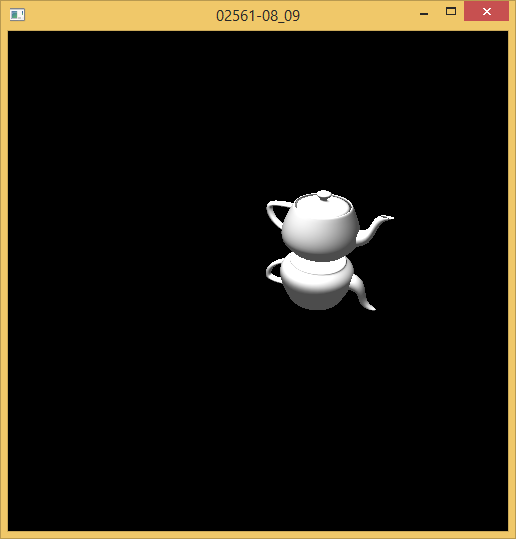
\includegraphics[width=8cm]{../Screenshots/ex-9b/3.png}
\caption{A teapot with a reflected teapot below}
\label{fig:9-3}
\end{figure}

\section{Part 4}

I manage to reflect the light by multiplying \emph{y} component of light position by minus one before rendering teapot and roll all changes back after rendering the reflection.

A screenshot of the scene after this implementation can be seen in Figure \ref{fig:9-4}

\begin{figure}[hp]
\centering
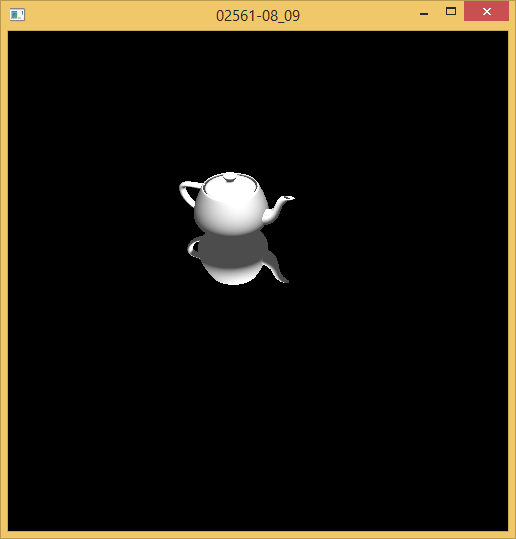
\includegraphics[width=8cm]{../Screenshots/ex-9b/4.png}
\caption{A teapot and its reflection with correct illumination}
\label{fig:9-4}
\end{figure}



\section{Part 5}

Firstly, I make the reflection teapot a little bit darker by multiplying its color with $0.5$ and I roll the change back after rendering the reflection teapot. After that, I enabled displaying the plane and blend the reflection with the plane. The blending process is carried out by this code fragment: \\

\begin{lstlisting}
glEnable (GL_BLEND);
glBlendFunc(GL_ONE,GL_ONE);
mat4 model;
drawMeshObject(projection,  model, view, 
    getLightViewProjection(),  planeObject);
    //renders the plane
glDisable(GL_BLEND);
\end{lstlisting}
\smallskip
\noindent
The resulting scene can be seen in Figure \ref{fig:9-5-1}.

\begin{figure}[hp]
\centering
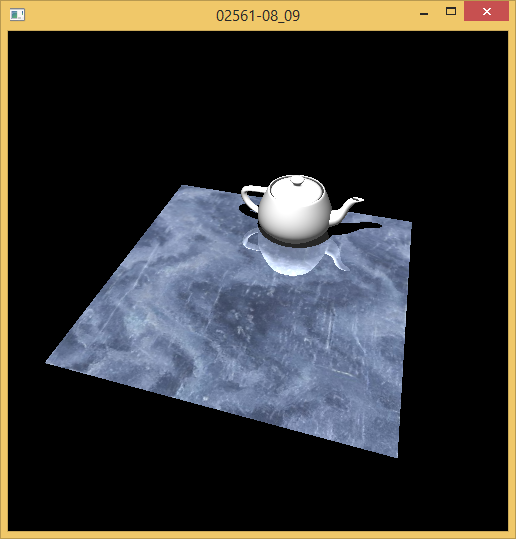
\includegraphics[width=8cm]{../Screenshots/ex-9b/5-1.png}
\caption{The teapot and its reflection on the plane}
\label{fig:9-5-1}
\end{figure}

However, there is a problem while rendering the teapot reflection. Parts of the reflection teapot that is above the plane should be cut out the scene. You can see a screenshot of the problem in Figure \ref{fig:9-5-2}. 


\begin{figure}[hp]
\centering
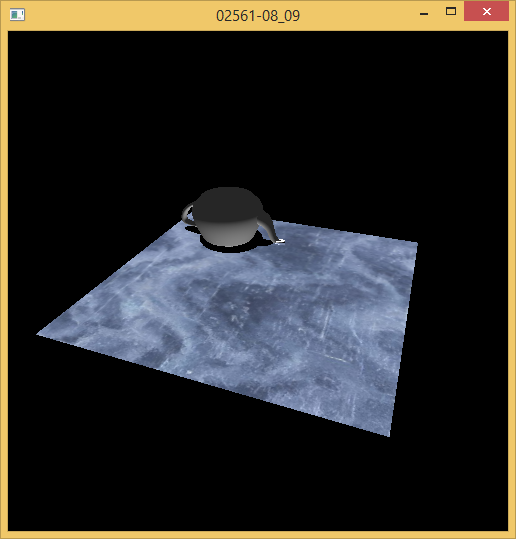
\includegraphics[width=8cm]{../Screenshots/ex-9b/5-2.png}
\caption{The planar reflection without introducing stencil buffer}
\label{fig:9-5-2}
\end{figure}

The solution of the problem is introduced in Part 6.

\section{Part 6}


Completion of this part is considered as a future work.

%%% Local Variables:
%%% mode: latex
%%% TeX-master: "report_main"
%%% End: 